\subsection{Interfaces}
\subsubsection{Syntax}
\begin{lstlisting}[style=C]
  public interface IList: Icollection, IEnumerable
  {
    int Add (object value);             //methods
    bool Contains(object value);        
    ...
    bool isReadOnly{get;}               //Property
    ...
    object this [int index]{get; set;}  //Indexer
    
  }
\end{lstlisting}
\begin{itemize}
  \item Ein Interface ist eine pure abstrakte Klasse $\rightarrow$ Nur
  Signaturen, keine Implementationen
  \item Kann Methoden, Properties, Indexers und Events enthalten
  \item Kann \textbf{nicht} Felder, Konstanten, Konstruktoren, Destruktoren,
  Operatoren oder nested Types enthalten. 
  \item Interface Members sind implizit public abstract (virtual)
  \item Interface Members dürfen nicht statisch sein
  \item Klassen und Strukts können mehrere Interfaces implementieren. 
  \item Interfaces können von anderen Interfaces erben
\end{itemize}

\subsubsection{Implementierung durch KLassen und Structs}
\begin{lstlisting}[style=C]
  class Myclass: MyBaseLcass, IList, ISerializable
  {
    public int Add (object value){...}
    public bool Contain (object value){...}
    ...
    public bool IsReadOnly {get {...}}
    ...
    public object this [int index] {get{...} set{...}}
  }
\end{lstlisting}
\begin{itemize}
\item Eine Klasse kann von einer einzelnen Basisklasse erben, kann aber mehrere
Interfaces implementieren. Ein Struct kann nicht von einem Type erben, aber
mehrere Interfaces implementieren. 
\item Jedes Interfacemember (Methode, Property, Indexer) muss aus einer
Basisklasse implementiert oder vererbt sein. 
\item Implementierte Interfacemethoden müssen \textbf{nicht} mit override
deklariert werden. 
\item Implementierte Interfacemethoden können als abstract deklariert werden.
(Ein interface kann also aus einer abstrakten Klasse implementiert werden)
\end{itemize}

\subsubsection{Working with Interfaces}
\begin{lstlisting}[style=C]
  //Zuweisungen: 
  MyClass c = new MyClass(); 
  IList list = c; 
  
  //Methoden-Aufruf:
  list.Add("Tom");  //Dynamic binding -> MyClass.Add
  
  //Type check:
  if(list is MyClass)       //True
  if(list is ISerializable) //True
  
  //Type casts: 
  c = list as MyClass; 
  c = (MyClass) list; 
  ISerializable ser = (ISerializable)list;
\end{lstlisting}

\subsubsection{Beispiel}
\begin{lstlisting}[style=C]
  interface ISimpleReader
  {
    int Read();  
  }
  
  interface IReader:ISimpleReader
  {
    void Open(string name); 
    void Close(); 
  }
  
  class Terminal: ISimpleReader
  {
    public int Read(){...}
  }
 
 class File: IReader
 {
  public int Read(){...}
  public void Open(string name){...}
  public void Close(){...}
 }
 
 ISimpleReader sr = null; 
 sr = new Terminal(); 
 sr = new File(); 
 
 IReader r = new File(); 
 sr = r; 
\end{lstlisting}
\begin{figure}[h]
  \centering
  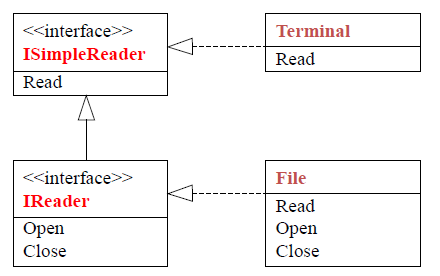
\includegraphics[height=5cm, ]{images/CSharp/InterfaceExample}
  \caption{Beispiel zu Interface} 
\end{figure}\\

\subsubsection{Name Clashes}
Siehe Beispiel auf Folie 6. 